%\documentclass[10pt,notes]{beamer}       % print frame + notes
%\documentclass[10pt, notes=only]{beamer}   % only notes
\documentclass[11pt]{beamer}              % only frames

%%%%%% IF YOU WOULD LIKE TO CREATE LECTURE NOTES COMMENT OUT THE FOlLOWING TWO LINES
%\usepackage{pgfpages}
%\setbeameroption{show notes on second screen=bottom} % Both

\usepackage{graphicx}
\DeclareGraphicsExtensions{.pdf,.png,.jpg}
\usepackage{color}
\usetheme{winslab}
\usepackage[utf8]{inputenc}
\usepackage[english]{babel}
\usepackage{amsmath}
\usepackage{amsfonts}
\usepackage{amssymb}





\usepackage{algorithm2e,algorithmicx,algpseudocode}
\algnewcommand\Input{\item[\textbf{Input:}]}%
\algnewcommand\Output{\item[\textbf{Output:}]}%
\newcommand\tab[1][1cm]{\hspace*{#1}}

\algnewcommand{\Implement}[2]{\item[\textbf{Implements:}] #1 \textbf{Instance}: #2}%
\algnewcommand{\Use}[2]{\item[\textbf{Uses:}] #1 \textbf{Instance}: #2}%
\algnewcommand{\Trigger}[1]{\Statex{\textbf{Trigger:} (#1)}}%
\algnewcommand{\Events}[1]{\item[\textbf{Events:}] #1}%
\algnewcommand{\Need}[1]{\item[\textbf{Needs:}] #1}%
\algnewcommand{\Event}[2]{\Statex \item[\textbf{On#1:}](#2) \textbf{do}}%
\algnewcommand{\Trig}[3]{\State \textbf{Trigger}  #1.#2 (#3) }%
\def\true{\textbf{T}}
\def\false{\textbf{F}}

\nocite{*}
\author[Ahmet Can Ogreten]{Ahmet Can Ogreten\\\href{mailto:ahmet.ogreten@metu.edu.tr}{ahmet.ogreten@metu.edu.tr}}
%\author[J.\,Doe \& J.\,Doe]
%{%
%  \texorpdfstring{
%    \begin{columns}%[onlytextwidth]
%      \column{.45\linewidth}
%      \centering
%      John Doe\\
%      \href{mailto:john@example.com}{john@example.com}
%      \column{.45\linewidth}
%      \centering
%      Jane Doe\\
%      \href{mailto:jane.doe@example.com}{jane.doe@example.com}
%    \end{columns}
%  }
%  {John Doe \& Jane Doe}
%}

\title[WINS Beamer Template]{Bracha-Toueg \& Chandra-Toueg Consensus Algorithms}
% \subtitle[Short SubTitle]{How to Prepare a Nice Presentation}
%\date{} 

\begin{document}

\begin{frame}[plain]
\titlepage
\note{In this talk, I will present .... Please answer the following questions:
\begin{enumerate}
\item Why are you giving presentation?
\item What is your desired outcome?
\item What does the audience already know  about your topic?
\item What are their interests?
\item What are key points?
\end{enumerate}
}
\end{frame}

\begin{frame}[label=toc]
    \frametitle{Outline of the Presentation}
    \tableofcontents[subsubsectionstyle=hide]
\note{ The possible outline of a talk can be as follows.
\begin{enumerate}
\item Outline 
\item Problem and background
\item Design and methods
\item Major findings
\item Conclusion and recommendations 
\end{enumerate} Please select meaningful section headings that represent the content rather than generic terms such as ``the problem''. Employ top-down structure: from general to more specific.
}
\end{frame}
%
%\part{This the First Part of the Presentation}
%\begin{frame}
%        \partpage
%\end{frame}
%
\section{Why We Need It ?}
%\begin{frame}
%        \sectionpage
%\end{frame}

\begin{frame}{Why We Need It ?}
Software needs to be resilient and fault-tolerant to ensure high availability. A typical setup includes at least three nodes to maintain service continuity.
% \framesubtitle{Tell a \alert{STORY} from the background to the conclusion}
\begin{block}{Consensus}
Multiple software entities must consistently communicate. When conflicts arise or an entity fails to respond, the remaining nodes must reach a decision using a consensus algorithm. This ensures system reliability despite failures or discrepancies.
\end{block}
Different situations demand specialized consensus algorithms to effectively manage communication and decision-making challenges in software systems.
\note{}
\end{frame}

\section{Bracha Toueg}
\begin{frame}{Bracha Toueg}
% \framesubtitle{}
\begin{figure}
    \centering
    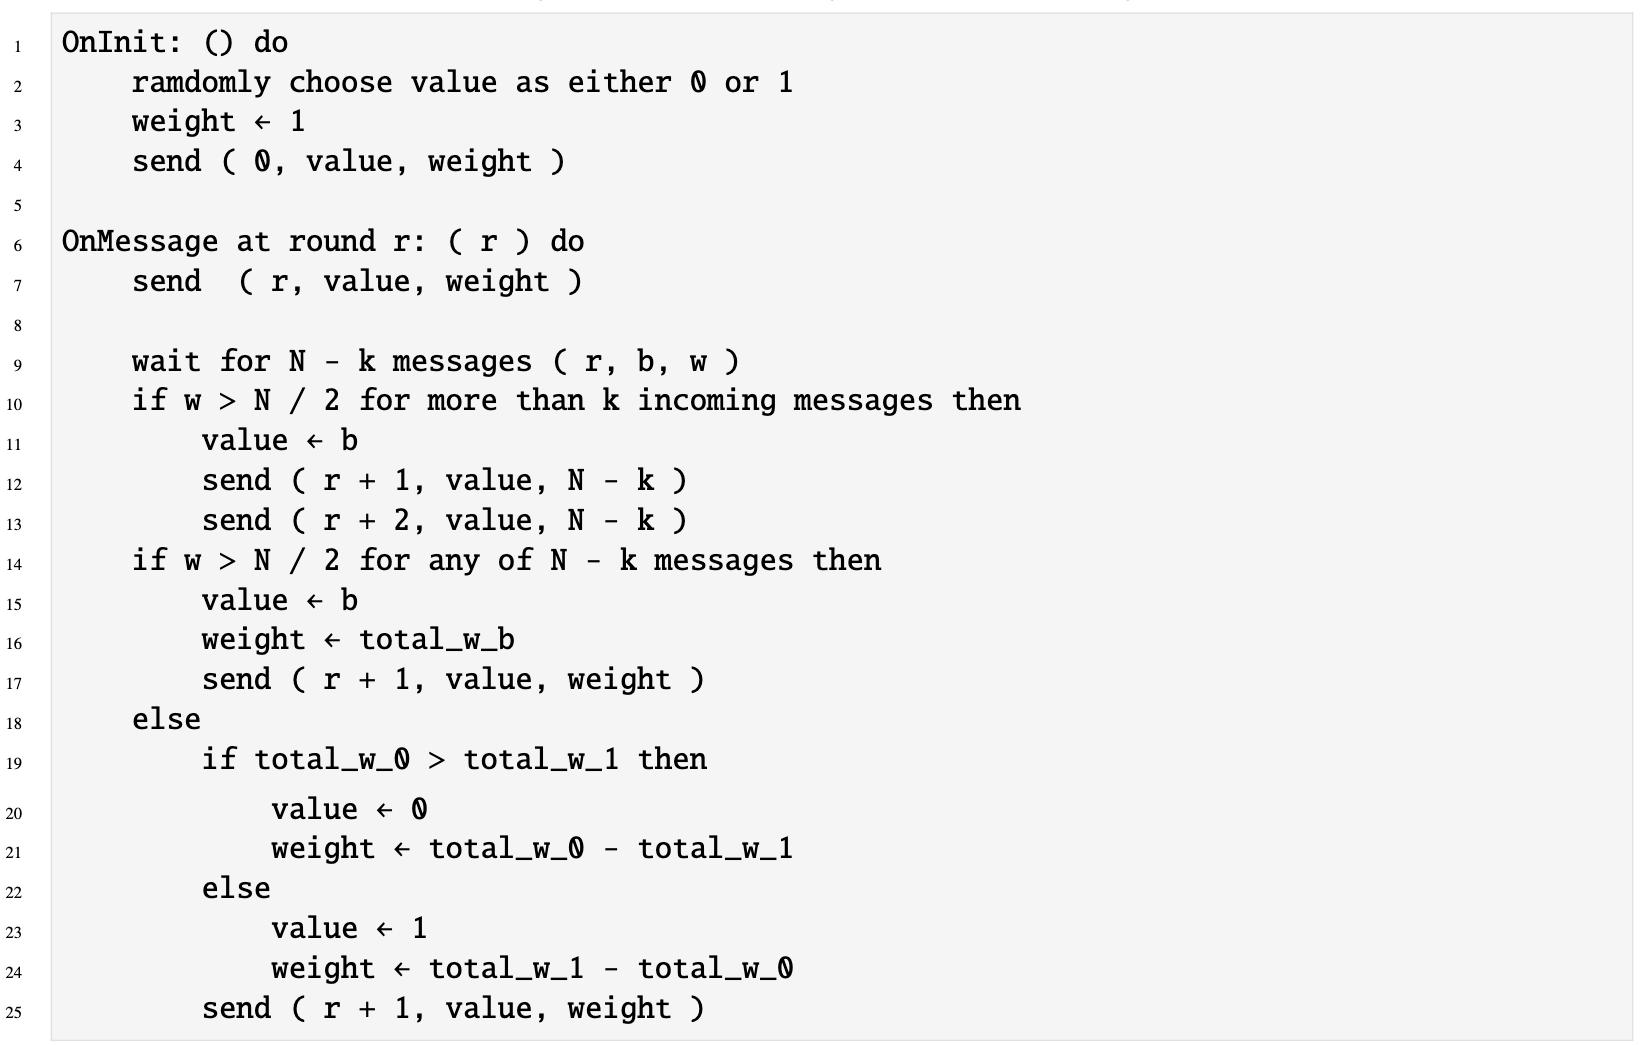
\includegraphics[scale=0.4]{bracha-toueg.png}
    \caption{Bracha Toueg Algorithm Sudo Code}
    \label{fig:bracha_toueg_sudo}
\end{figure}

% Explain \textbf{YOUR} contributions. Go top-down. Give the brief introduction to the contributions at the beginning of the presentation. A slide should have no more than five to six lines of text or bullets. Prefer figures instead of text: A picture is worth a thousand words.
% \begin{itemize}
% \item Communicate the Key Ideas
% \item Don’t get Bogged Down in Details
% \item Use a Top-down Approach
% \end{itemize}

% The audience will remember at most one single message \textbf{Which message you want to audience to remember? Can you express this message in less than a minute in an elevator?}

\end{frame}

\subsection{An Example}
\begin{frame}{Bracha Toueg}
\framesubtitle{An example}
Given a network of three processes p, q, r, and k = 1.

\begin{itemize}
\item Initially, p and q randomly choose the value 0 and r the value 1, all three with weight 1.
\item In round 0, p takes into account the messages from p and r; it sets its value to 1, and its weight to 1. Moreover, q and r both take into account the messages from p and q; they set their value to 0, and their weight to 2
\item  In round 1, q takes into account the messages from q and r; since both messages carry weight 2, it decides for 0.
\end{itemize}
\end{frame}


\begin{frame}{Bracha Toueg}
\framesubtitle{An example (contd.)}
\begin{itemize}
\item Moreover, p and r both take into account the messages from p and r; since the message from r carries weight 2, they set their value to 0, and their weight to 1.
\item At the start of round 2, q crashes. So p and r can take into account only the messages from p and r; as a result, they set their value to 0, and their weight to 2.
\item In round 3, p and r can again only take into account the messages from p and r; since both messages carry weight 2, they decide for 0.
\item p and r send messages with value 0 and weight 2 for two more rounds, and terminate.
\end{itemize}

\end{frame}

\subsection{Correctness}
\begin{frame}{Bracha Toueg}
\framesubtitle{Correctness}
\begin{itemize}
\item If scheduling of messages is fair, then the Bracha-Toueg k-crash consensus algorithm, for any \(k < N/2\) , is a Las Vegas
algorithm that terminates with probability one.
\item Proved in \cite{Fokking2013}\alert{Fokking2013}.
\end{itemize}
\end{frame}

\subsection{Complexity}
\begin{frame}{Bracha Toueg}
\framesubtitle{Complexity}
\begin{itemize}
    \item Each round of the algorithm involves every non-faulty process broadcasting its current state (value and weight) to all other processes.
    \item The number of messages transmitted in each round is \(O(n^2)\).
    \item If up to k processes may fail, the algorithm still requires messages from at least N-k processes to proceed, maintaining the \(O(n^2)\) complexity per round
    \item Computational complexity includes evaluating received messages to update weights and potentially decide on a value if conditions are met, which is \(O(n)\) per process per round.
\end{itemize}
\end{frame}

\section{Chandra Toueg}
\begin{frame}{Chandra Toueg}
\begin{figure}
    \centering
    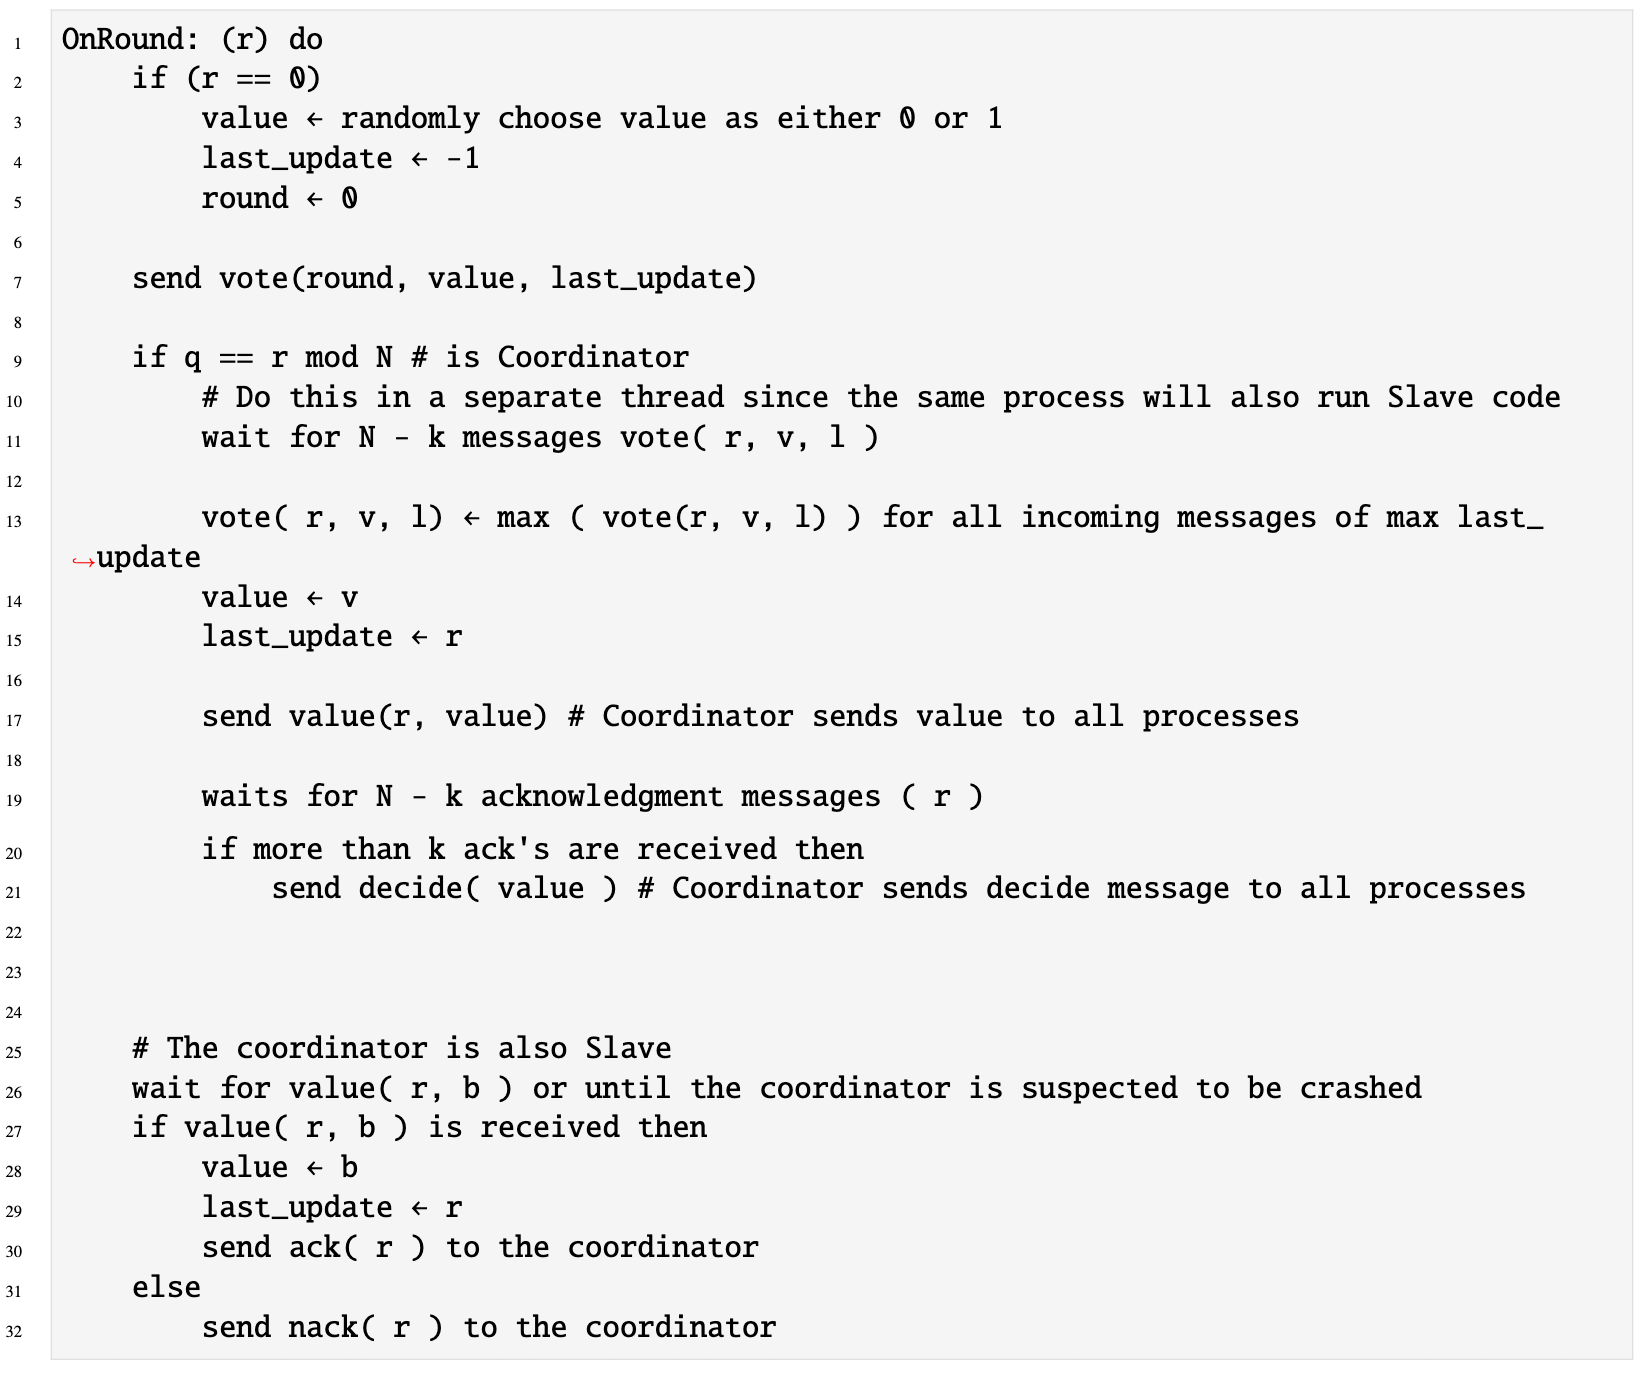
\includegraphics[scale=0.3]{chandra-toueg.png}
    % \caption{Chandra Toueg Algorithm Sudo Code}
    \label{fig:chandra_toueg_sudo}
\end{figure}
% \framesubtitle{}
% Explain \textbf{YOUR} contributions. Go top-down. Give the brief introduction to the contributions at the beginning of the presentation. A slide should have no more than five to six lines of text or bullets. Prefer figures instead of text: A picture is worth a thousand words.
% \begin{itemize}
% \item Communicate the Key Ideas
% \item Don’t get Bogged Down in Details
% \item Use a Top-down Approach
% \end{itemize}

% The audience will remember at most one single message \textbf{Which message you want to audience to remember? Can you express this message in less than a minute in an elevator?}

\end{frame}

\begin{frame}{Chandra Toueg}
\framesubtitle{An Example}
Given a complete network of three processes \(p_0, p_1, p_2\), and \(k = 1\)

\begin{itemize}
\item Initially, \(p_0\) and \(p_2\) randomly choose the value 1 and \(p_1\) the value 0; last-update=-1 at all three processes.
\item In round 0, the coordinator \(p_0\) takes into account the messages from \(p_0\) and \(p_1\), selects the message from
\(p_1\) to determine its new value, and broadcasts the value 0. When \(p_0\) and \(p_1\) receive this message, they set
their value to 0 and last-update to 0, and send ack to \(p_0\); moreover, \(p_1\) moves to round 1.
\item However, \(p_2\) moves
to round 1 without waiting for a message from \(p_0\), because its failure detector falsely suspects that \(p_0\) has
crashed; \(p_2\) sends nack to \(p_0\), and moves to round 1. The coordinator \(p_0\) receives the ack’s of \(p_0\) and \(p_1\),
decides for 0, and crashes before it can broadcast a decide message.
\end{itemize}
\end{frame}

\subsection{An Example}
\begin{frame}{Chandra Toueg}
\framesubtitle{An Example (contd.)}
\begin{itemize}
\item In round 1, the coordinator \(p_1\) can take into account only the messages from \(p_1\) and \(p_2\). It must select the
message from \(p_1\) to determine its new value, because it has the highest last-update. So \(p_1\) broadcasts the value
0. 
\item When \(p_1\) receives this message, it sets its value to 0 and last-update to 1, and sends ack to itself. The process
\(p_2\) moves to round 2 without waiting for a message from \(p_1\), because its failure detector falsely suspects that
\(p_1\) has crashed; \(p_2\) sends nack to \(p_0\), and moves to round 2. After \(p_1\) has received the ack and nack from
\(p_1\) and \(p_2\), respectively, it also moves to round 2.
\end{itemize}
\end{frame}

\begin{frame}{Chandra Toueg}
\framesubtitle{An Example (contd.)}
\begin{itemize}
\item In round 2, the coordinator \(p_2\) can take into account only the messages from \(p_1\) and \(p_2\). It must select the
message from \(p_1\) to determine its new value, because it has the highest last-update. So \(p_2\) broadcasts the value
0. When \(p_1\) and \(p_2\) receive this message, they set their value to 0 and last-update to 2, and send ack to \(p_2\);
moreover, \(p_1\) moves to round 3.
\item The coordinator \(p_2\) receives the ack’s of \(p_1\) and \(p_2\), decides for 0, and
broadcasts \(<decide, 0>\). When \(p_1\) receives this message, it also decides for 0.
\end{itemize}
\end{frame}

\subsection{Correctness}
\begin{frame}{Chandra Toueg}
\framesubtitle{Correctness}
\begin{itemize}
\item A failure detector is called \alert{eventually weakly accurate} if from some point in time on, some correct process is never
suspected by any process.
\item In the presence of an eventually weakly accurate failure detector, the Chandra-Toueg algorithm is an (always correctly
terminating) k-crash consensus algorithm for any \(k < N/2\).
\item Proved in \cite{Fokking2013}\alert{Fokking2013}.
\end{itemize}
\end{frame}

\subsection{Complexity}
\begin{frame}{Chandra Toueg}
\framesubtitle{Complexity}
\begin{itemize}
\item \alert{Time complexity of a round:}The number of rounds of the protocol is bounded by n, when used with a failure detector
of the class S. There is no upper bound when it is used with a failure detector of the class \(<>S\).
\item \alert{Message complexity of a round:}During each round, each process sends a message to eachprocess (including itself).
Hence, the message complexity of a round is upper bounded by \(n^2\)
\item \alert{Message type and size:}There are two types of message: \alert{est} and \alert{decide}. A decide message carries only a proposed
value. An est message carries a proposed value (or the default value)plus a round number. The size of the round number
is bounded by \(log_2(n)\) when the underlying failure detector belongs to S. It is not bounded in the other case
\item Explained in \cite{Mostefaoui1999}\alert{Mostefaoui1999}.
\end{itemize}
\end{frame}

\section{Experimentation Results for Chandra Toueg}

\subsection{Methodology}
\begin{frame}{Experimentation Results for Chandra Toueg}
\framesubtitle{Methodology}
\begin{itemize}
\item The topology for the experiment is considered completely connected. It is assumed that the failure detector module will
not detect any other process as crashed during execution of the consensus algorithm
\item The detector module
in process p populates \(D_p\) randomly before consensus algorithm starts execution.
\item As \cite{Hossain}\alert{Hossain} depicted in his research
\end{itemize}
\end{frame}

\begin{frame}{Experimentation Results for Chandra Toueg}
\framesubtitle{Methodology (contd.)}
\begin{itemize}
\item Three parameters are measured to analyzed the performance of the algorithm:
\begin{enumerate}
    \item The average number of round needed
to receive all processs values for different number of Processes in the system. The algorithm is run for N = 4, 8, 12,
··· 60.    
    \item For each round, the percentage of processes that get values from all other processes. In this case,
N = 8 and 60 is considered to show the comparison result for the parameter
    \item Average number of waiting time for
each process in phase1 for N =8 and 60. Waiting time is the number of times a presses is selected to execute but has to
wait to receive all processes’ values who are not in its \(D_p\).
\end{enumerate}
\end{itemize}
\end{frame}

\subsection{Results}
\begin{frame}{Experimentation Results for Chandra Toueg}
\framesubtitle{Results}
\begin{enumerate}
\item The average number of round needed
to receive all processs values for different number of Processes in the system. The algorithm is run for N = 4, 8, 12,
··· 60.
\end{enumerate}
\begin{figure}
    \centering
    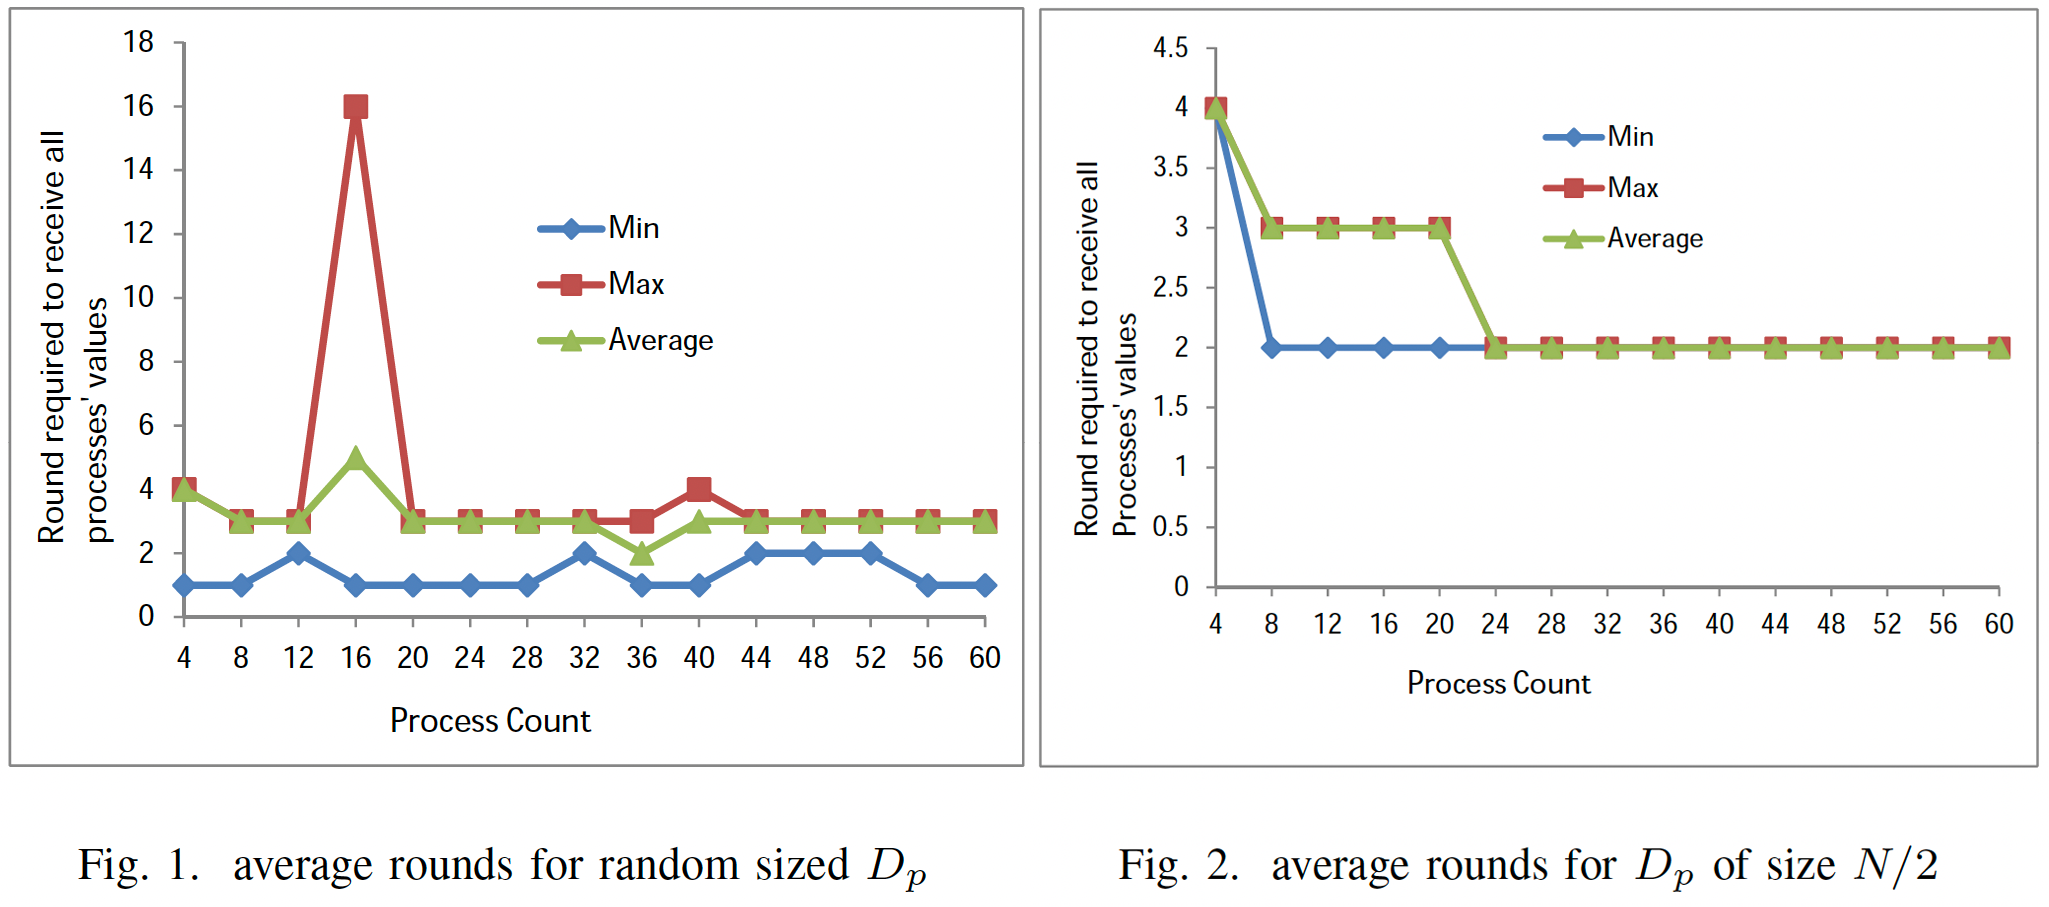
\includegraphics[scale=0.3]{fig1.png}
    % \caption{Chandra Toueg Algorithm Sudo Code}
    \label{fig:chandra_toueg_sudo}
\end{figure}
\end{frame}

\begin{frame}{Experimentation Results for Chandra Toueg}
\framesubtitle{Results (contd.)}
    \begin{enumerate}
    \setcounter{enumi}{1}
    \item For each round, the percentage of processes that get values from all other processes. In this case,
    N = 8 and 60 is considered to show the comparison result for the parameter.
\end{enumerate}
\begin{figure}
    \centering
    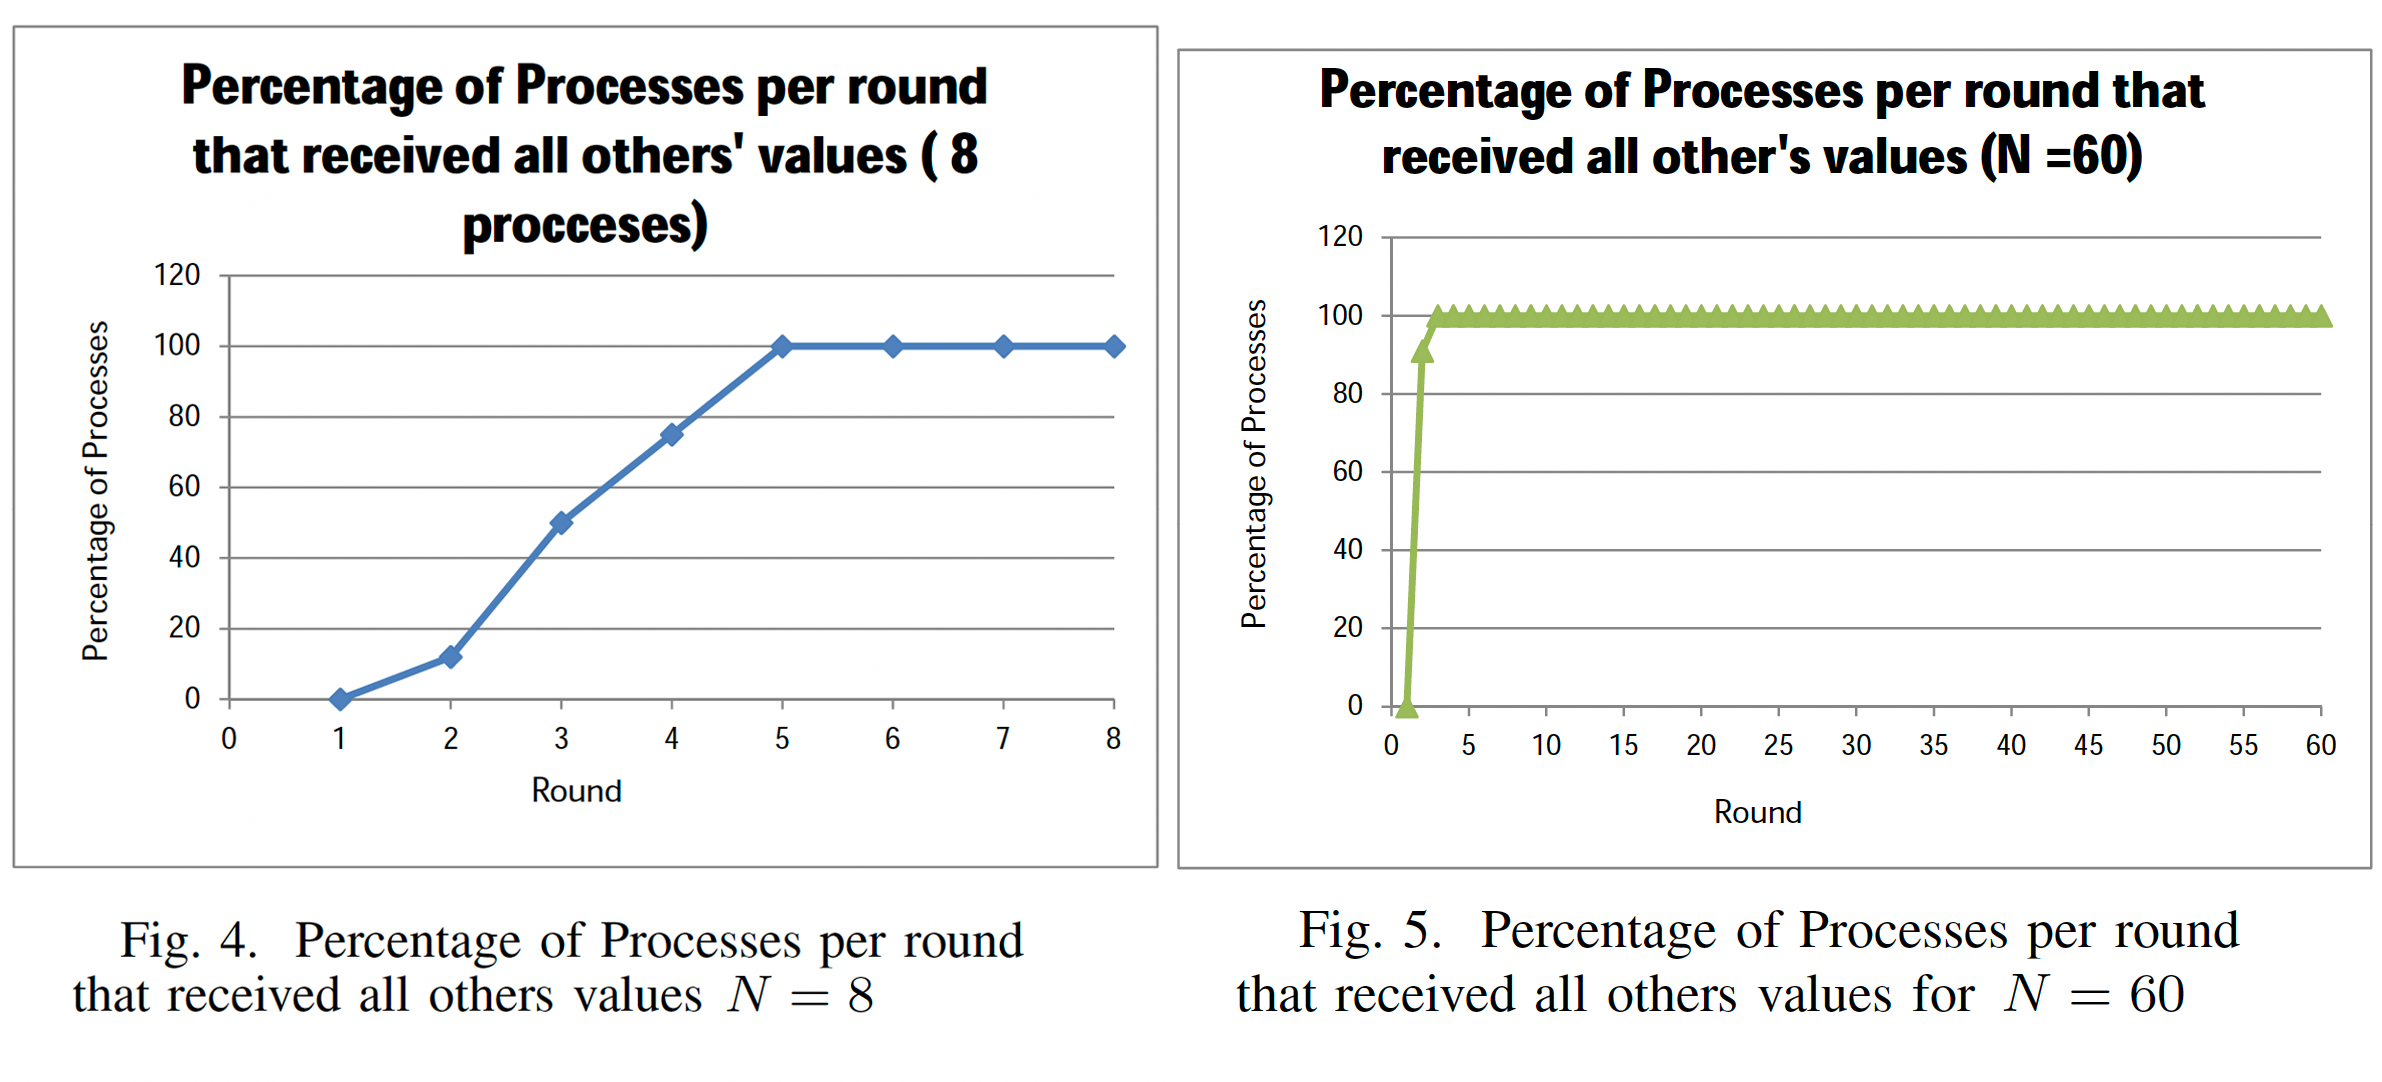
\includegraphics[scale=0.25]{fig4.png}
    % \caption{Chandra Toueg Algorithm Sudo Code}
    \label{fig:chandra_toueg_sudo}
\end{figure}
\end{frame}

\begin{frame}{Experimentation Results for Chandra Toueg}
\framesubtitle{Results (contd.)}
\begin{enumerate}
\setcounter{enumi}{2}
\item Average number of waiting time for
each process in phase1 for N =8 and 60. Waiting time is the number of times a presses is selected to execute but has to
wait to receive all processes’ values who are not in its \(D_p\).
\end{enumerate}
\begin{figure}
    \centering
    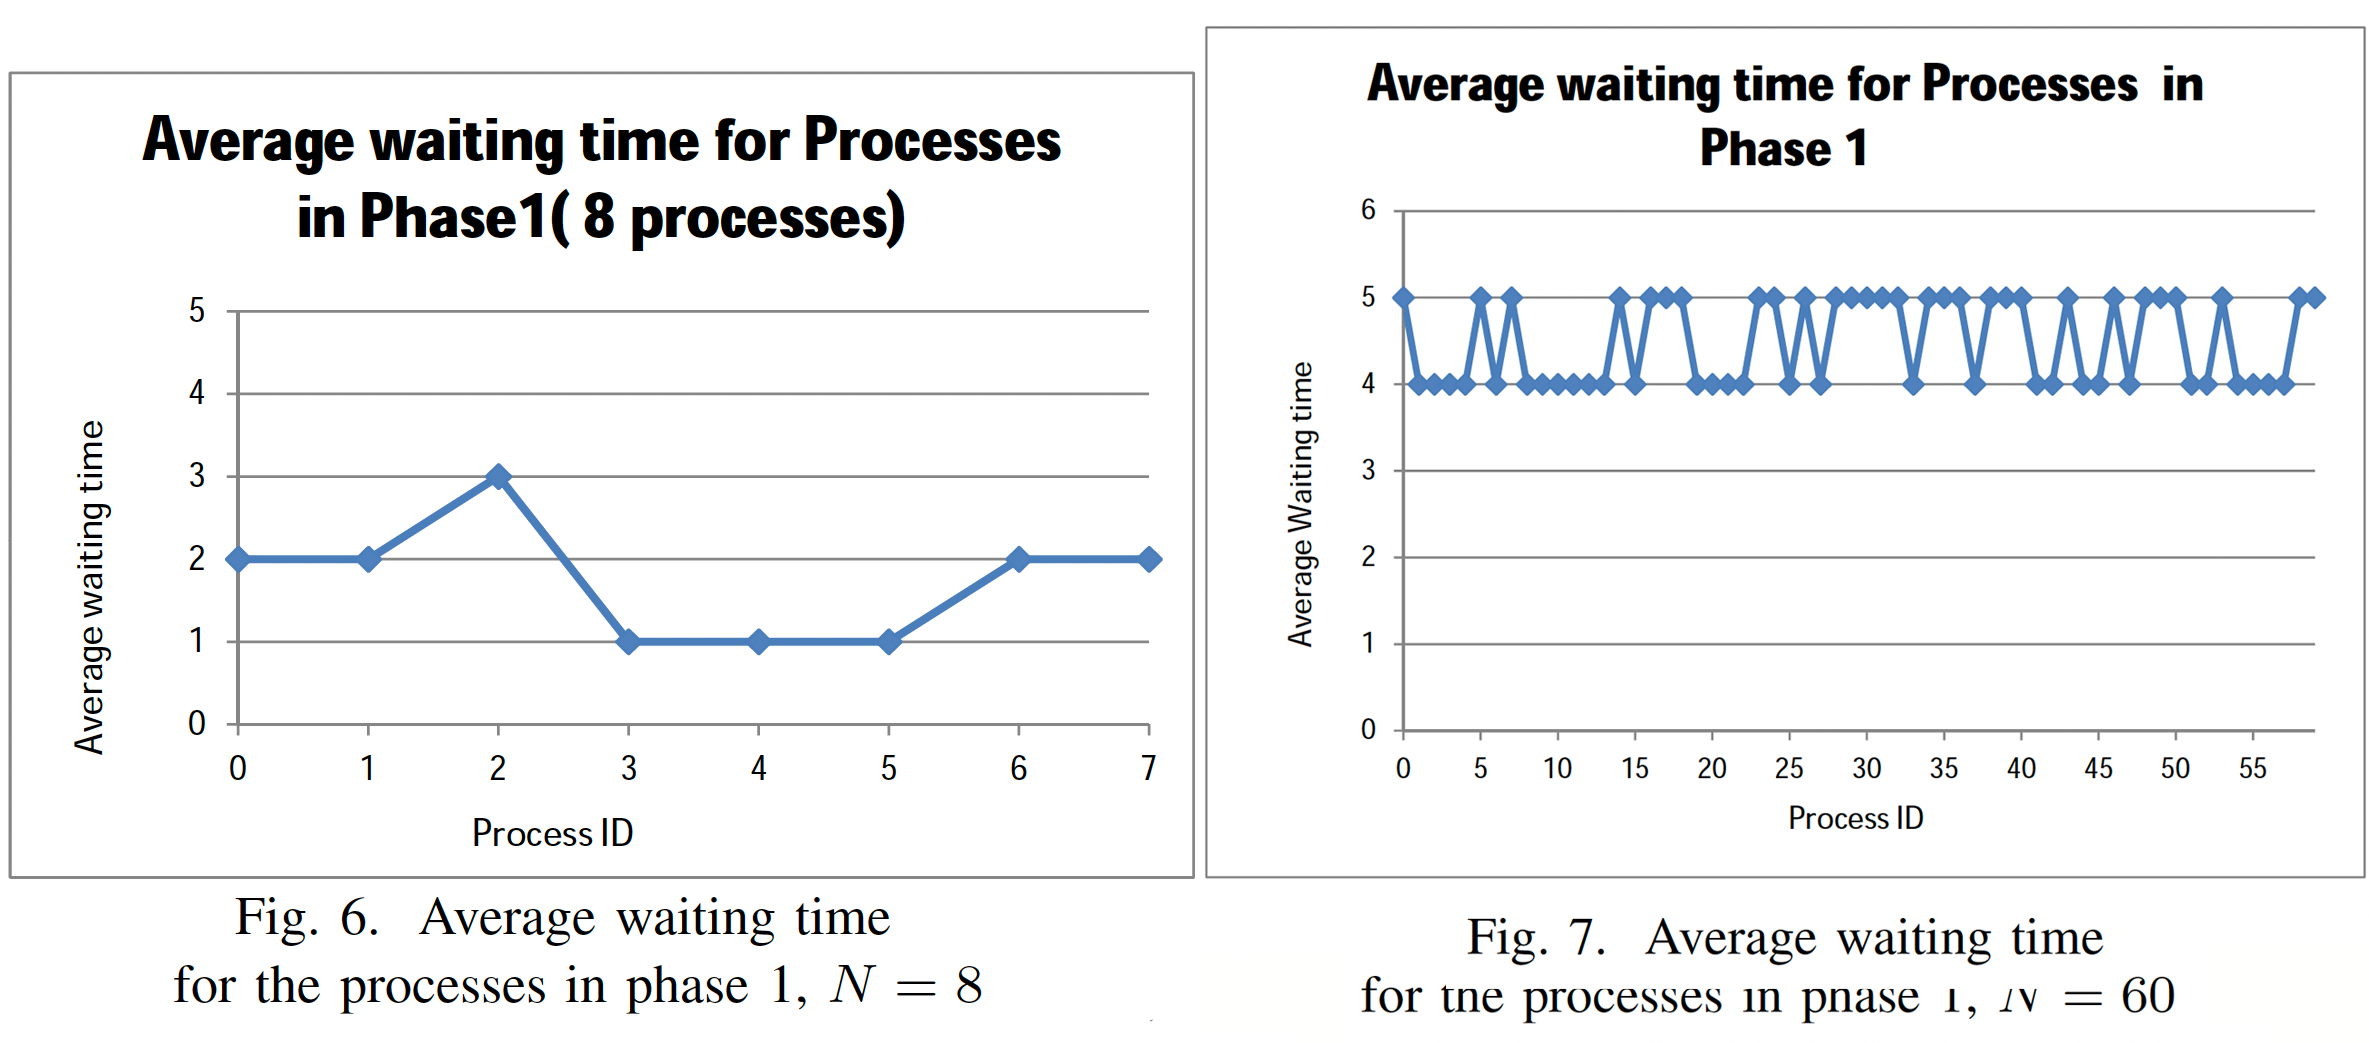
\includegraphics[scale=0.25]{fig6.png}
    % \caption{Chandra Toueg Algorithm Sudo Code}
    \label{fig:chandra_toueg_sudo}
\end{figure}
\end{frame}

\section{Conclusion} % When To Use Which ?
\begin{frame}{Conlusion}
\framesubtitle{}
\begin{itemize}
\item \alert{Chandra-Toueg:} Best in stable environments with reliable failure detectors. It excels in scalability but depends heavily on detector accuracy, limiting its use in dynamic networks.
\item \alert{Bracha-Toueg:} Effective without failure detectors, robust in environments with predictable crash limits. Ideal for critical systems needing resilience under communication delays.
\item \alert{Key Takeaway:} Select algorithms based on network stability and system needs. Future research could develop adaptive, hybrid models to enhance fault tolerance and reduce operational complexity.
\end{itemize}
\end{frame}


\section*{References}
\begin{frame}{References}
\tiny
\bibliographystyle{IEEEtran}
\bibliography{refs}
\end{frame}


\thankslide




\end{document}